\section{Methodology}

In this section the subsection environment will explain which tools were used to program the autoencoders
and which hardware the developed models were trained and written on. The subsection Datasets 
contains information about the remote sensing image data that was analyzed using the autoencoders. 
The architecture subsection lays out 
the design of the different models regarding the layers and loss functions. The last subsection, 
Latent Space, explains the technique used to visualize and understand the latent code between the 
encoder and decoder with comparisons of the latent space between different architectures and varying
sizes of the latent code.

\subsection{Environment}

\subsubsection{Hardware}

Training autoencoders with larger images of multiple channels takes a lot of computation especially if the 
features that should be learned are as complicated and abstract as the topography of remote sensing data.
As this is very time consuming the training of the models was mainly done on a remote machine from the
Leibniz University in Hannover that could run 24/7. Only the
programming of the models and tests with small datasets took place on a local personal computer that had no
GPU that was capable of training models in the given scenario. The following
are the specifications of the used systems:\\

\paragraph{Personal Computer} \mbox{} \smallskip \\

AMD Ryzen 7 1700, 16 GB RAM, NVIDIA GeForce GTX 760 2GB

\paragraph{Remote Machine} \mbox{} \smallskip \\

Lenovo Legion Y520T-25IKL, Intel i7-7700, 8GB RAM, NVIDIA GeForce GTX 1060 3GB

\subsubsection{Software}

The programming language used for the work is Python \parencite{1995-rossum-python} with the development
environment PyCharm locally
and and Jupyter Notebooks on a remote machine. The machine learning framework Tensorflow was used which
is developed by Google and offers cross-platform support, running on most CPUs and GPUs 
\parencite{2015-martin-tensorflow}.
Whenever possible Tensorflow's implementation of the Keras API specification was used which is a high level API
for training machine learning models. For dimensionality reduction of the latent space, Scikit-Learn was used
\parencite{2011-pedregosa-scikit}.

\subsection{Datasets} \label{datasets}

The available data are 1024x1024 images of the two United States cities Jacksonville
in Florida and Omaha in Nebraska taken from the US3D Dataset that
was partially published to provide research data for the problem
of 3D reconstruction \parencite{2019-bosch-semantic}.
The images for each recorded area cover one square kilometer and can be divided 
into four categories with the first one being multispectral satellite images with eight channels (MSI). 
From the MSI data three channels were extracted and used as red, green and blue intensities (RGB). 
Thirdly there are digital surface models (DSM) and Lastly semantic labeling with five different categories. \\

The MSI data was collected by the WorldView-3 satellite of Digital Globe from 2014 to 2016.
The images were taken in different seasons and times of day leading to great differences
in their appearance regarding for instance shadows, reflections, overall brightness or clouds.
This is an advantage for training models that are capable of processing data with similar differences in 
appearance.
In the MSI dataset a single picture consists of eight channels for eight different bands of the spectrum with
a ground sample distance of 1.3 meters. The eight channels of the imagery correspond to the following wavelengths:

\begin{tabular} {c c}
    \parbox{5cm}{
        \begin{itemize}
            \item Coastal: 400 - 450 nm 			
            \item Blue: 450 - 510 nm			
            \item Green: 510 - 580 nm 			
            \item Yellow: 585 - 625 nm
        \end{itemize}
    }
    \parbox{5cm}{
        \begin{enumerate} 			
            \item Red: 630 - 690 nm
            \item Red Edge: 705 - 745 nm
            \item Near-IR1: 770 - 895 nm
            \item Near-IR2: 860 - 1040 nm
        \end{enumerate}
    }
\end{tabular}
\bigskip

Three of those channels were extracted and used as RGB data. 
Each pixel of an image is described by three bytes representing the intensity of the wavelengths of the 
reflected light corresponding to either red, green or blue.

The DSM data was collected using light detection and ranging technology (Lidar) which measures the 
distance to points of the earth's surface. This distance is proportional to the value of the single channel
that each pixel of the DSM has.

Lastly, there are semantically labeled pictures with one channel of a single byte that encodes one of five 
different topographic classes. Those classes are vegetation, water, ground, building and clutter. 
The semantic labeling was done automatically from lidar data but manually checked and corrected afterwards.

Those four categories of data all cover one square kilometer in each image.
Additionally they contain a lot of oblique view on buildings and other valuable
features like clear shadows making the data ideal for training models that should 
detect those features.

In the dataset there are $2,783$ $1024\times 1024$ RGB images available. Since the autoencoder should
be able to distinguish between categories like shadows and vegetation each image is split into $64$
$128\times 128$ pictures resulting in $178,112$ total training images. 
Experimentation with larger image dimensions never produced reconstructions of acceptable
quality regarding pure visual inspection.
Another option would be to resize larger sections of the original images to $128\times 128$. However,
smaller picture sections
are more likely to have a dominant feature like containing mainly shadows, buildings or vegetation.
This is desirable since the variational autoencoder should learn to distinguish those features and to cluster
them in an unsupervised manner.


\subsection{Architecture} \label{architecture}

The first general structure of the vanilla autoencoder and the variational autoencoder is a combination 
of the convolutional autoencoder and the variational autoencoder presented in the second edition of
Hans-On Machine Learning \parencite{2017-geron-homl}.
That model is adjusted to work with $128\times 128$ RGB images and various different architectural
changes are tested. These experiments are first conducted with only $3000$ training images and $200$ validation
images since the training should be fast to allow testing many different architectures. The best performing
models are then evaluated and compared after training with all $178,122$ pictures. 
Here the performance is measured regarding the quality of the reconstruction and not the quality of the latent space.
In all these test the dimension
of the latent code is $1024$ while the architectures allow to alter the coding size for the experiments regarding
the latent space \ref{latent_space_experiments}. The described experiments regarding the architecture and their
evaluation can be found
in section \ref{architecture_experiments}.

The results were that a purely convolutional network without pooling performed the best. However, to inspect the 
effects of pooling on the latent code an architecture with pooling is used as the second model in the latent space
experiments. This model yields results that are only a little worse than the ones from the purely convolutional
network but the training times were almost twice as long.\\

The following are choices that apply to both architectures. The RGB input values between 0 and 255 are first 
normalized. Each value is divided by $255$ which way there are only floats between $0$ and $1$.
The last deconvolutional layer in the decoder network (Figure \ref{figure_decoder}) uses the sigmoid activation
function $S(x) = \frac{e^x}{e^x+1}$. This guarantees that the values in the output image are all 
between $0$ and $1$ and can be interpreted as RGB values. 
Every other layer uses a scaled exponential linear unit (SELU) as activation function with the standard scale
$\lambda = 1.05070098$ and $\alpha = 1.67326324$ as they were calculated in \parencite{2017-klambauer-selu}.
This choice is made based on the insights from related work \ref{related_work_general_architecture}.

\begin{equation}
    selu(x) = \lambda \begin{cases}
        x & if x > 0 \\
        \alpha e^x- \alpha & if x \leq 0
    \end{cases}
\end{equation}

\subsubsection{Pure Convolutional Architecture} \label{section_pure_convolutional_architecture}

Figure \ref{figure_pure_convolutional_encoder} visualizes the used encoder network. It has an example size for the
latent code of $1024$ which is not fixed. There are three convolutional
layers with kernels of the dimension $3\times 3$ and strides of two. The output of the last convolutional layer
is flattened to a single vector which means that it has the size of the depth times the height times the width of
the last convolutional layer, i. e. $32*16*16 = 8,192$. This flattened vector is the input for two fully connected
dense layers that produce the means and standard deviations with the chosen size of the latent code. The final step
is to sample the latent code from the means and deviations.

\begin{figure}[h]
    \centering
    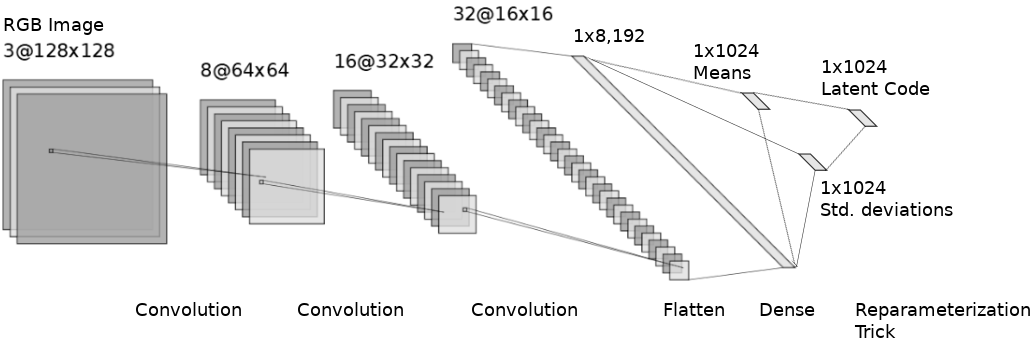
\includegraphics[width=\textwidth]{images/figures/encoder_neural_network.png}
    \caption{Encoder network architecture with an encoding size of 1024.
    The kernel size is $3\times 3$ in every layer. The 
    reparameterization trick in the last layer
    refers to the sampling as described in section \ref{vae_background}.
    Dimensions are specified as $depth@height\times width$.} \label{figure_pure_convolutional_encoder}
\end{figure}

The decoder, as visualized in Figure \ref{figure_decoder}, takes the latent code produced by the encoder and 
first passes it through a dense layer with a $32*16*16=8,192$ output. This way it is possible to reshape that
output vector to $32\times 16\times 16$ as the next step. After that three deconvolutions are applied.
These deconvolutional layers are symmetrical to the convolutional layers in the first network resulting in an 
output with the same dimensions as the input of the encoder. 

\begin{figure}[h]
    \centering
    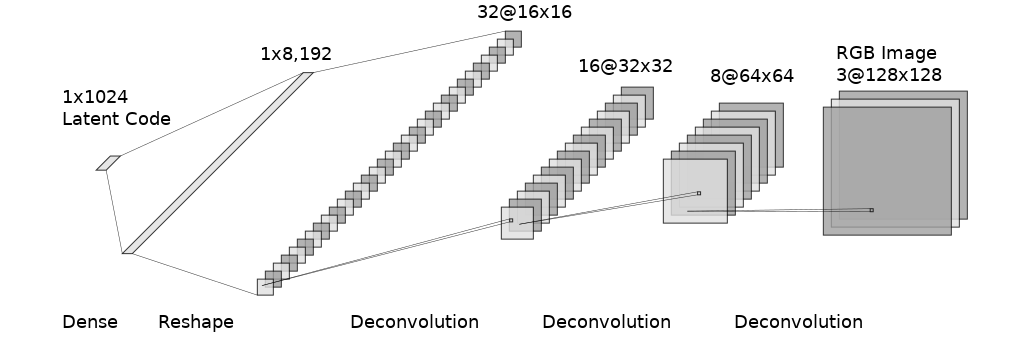
\includegraphics[width=\textwidth]{images/figures/decoder_neural_network.png}
    \caption{Decoder network architecture with an encoding size of 1024.
    The kernel size is $3\times 3$ in every layer. The last deconvolutional layer has a sigmoid activation
    function. Dimensions are specified as $depth@height\times width$.} \label{figure_decoder}
\end{figure}

\subsubsection{Max Pooling Architecture}

The used encoder with max pooling is depicted in Figure \ref{figure_encoder_pooling}. It contains three
convolutional and three pooling layers with a pooling layer following every convolutional layer. The convolutional
kernels have size $3\times3$ and the convolution is done with strides of one which means that they do not reduce
height and width of their input. Instead each pooling layer quarters the dimension with a pooling window of size
$2\times 2$. This produces and output of size $32\times16\times16$ that is processed further in the same way
as in the pure convolutional encoder \ref{section_pure_convolutional_architecture}.
The decoder is also equivalent to the one in the pure convolutional architecture.

\begin{figure}[h]
    \centering
    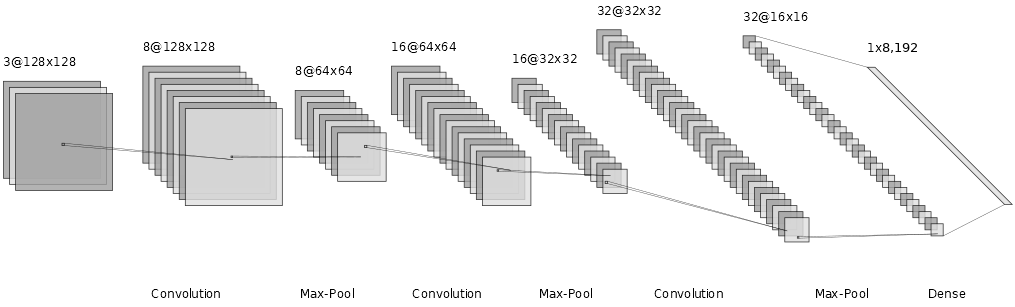
\includegraphics[width=\textwidth]{images/figures/encoder_pooling.png}
    \caption{Part of the encoder network architecture with pooling and an encoding size of 1024.
    The convolutional kernel always has size $3\times 3$. The pooling window always has size $2\times 2$.
    The rest of the encoder that generates the latent code is the same as in the fully convolutional encoder
    \ref{section_pure_convolutional_architecture}.
    Dimensions are specified as $depth@height\times width$.} \label{figure_encoder_pooling}
\end{figure}

\subsection{Understanding Latent Space}

To understand and work with the latent space learned by the variational autoencoder is problematic and
difficult since it is a very high dimensional space and it is not known which information of the input the
autoencoder learns. For the understanding and visualization of the latent space its dimensionality needs
to be reduced while preserving the underlying structure of the latent space. Then the low dimensional
codes can be visualized in a way that allows humans to comprehend what the autoencoder learned.
One dimensionality reduction method that could be used here is principal component analysis (PCA).

However,
t-distributed stochastic neighbor embedding (t-SNE), as presented in \ref{t-sne}, is the technique used in this work.
The reason for this choice is that PCA focuses on preserving large distances, so dissimilar points in the
high dimensional space appear far apart in a low dimensionality visualization. For visualization though
it may be more interesting to keep more of the underlying structure which is accomplished by t-SNE as its
focus is on preserving the context of points to their neighbors \parencite{2008-vanDerMaaten-visualizing}.
That behavior is caused by the asymmetry of the used Kullback-Leibler divergence \ref{KL-Divergence}.
During the training process it penalizes a lot if large probabilities, i. e. far apart points, in high dimensional
space are represented by small probabilities, i. e. close together points, in low dimensional space. Meanwhile, the 
penalty is negligible if small probabilities in high dimensional space are represented by large probabilities in
low dimensional space, leading to the claimed focus on local similarities.

After t-SNE is used to reduce the dimensions of the latent code to 2, the low dimensional representation can be
plotted in a scatter plot. That way it becomes evident if the autoencoder has learned any distinct clusters.
To recap, every point in those plots is a low dimensional representation of a latent code that corresponds to
a $128 \times 128$ section of an RGB satellite image. 
Now the goal is to find out what features the learned clusters in the plots correspond to. For that purpose the
semantic labeling and digital surface models \ref{datasets} are used. In the first type of plot the points
are colored according to the most dominant class in the corresponding image. Those classes are building, vegetation,
water, ground and clutter. In the second kind of plot the points have a gray value equal to the average pixel
values in the digital surface models meaning that points for images, that have on average more heights, are brighter
than points representing images with less heights.
In these two types of plots the points are squares if the related image is from Jacksonville or circles if it is from
Omaha. In a third type of plot the points are represented by the corresponding images themselves 

In those plots it can be observed if the clusters correlate to one of the visualized features which would mean that
the autoencoder has learned to cluster that feature.
This method is repeated for different coding sizes for the two architectures presented in \ref{architecture}.
That process gives insight into what coding sizes yield the best unsupervised clustering. The specific experiments
and results are found in the experiments section \ref{latent_space_experiments}.
